\section{Materials and Methods}

\subsection{Datasets}

Three datasets were evaluated (Table~\ref{tab:datasets}): Ames bacterial reverse mutation 
($n = 13{,}560$), in-vitro chromosome aberration ($n = 1{,}619$), and in-vivo micronucleus 
($n = 2{,}153$).

The Ames dataset combines pharmaceutical (drug-like) and industrial chemical sources. 
Drug-sourced compounds were obtained from the Hansen benchmark\cite{Hansen_2009} and the 
Honma/Furuhama Ames/QSAR Challenge datasets,\cite{Honma_2019,Furuhama_2023} which were 
curated by the original authors using literature-derived Ames assay results without 
additional Klimisch filtering applied here; these benchmarks are intentionally enriched for 
known mutagens for evaluation purposes, which contributes to their elevated positive rate. 
Industrial-sourced compounds were obtained from ECHA REACH dossiers and K-REACH 
submissions, then filtered by Klimisch reliability score (see below). Compounds carry a 
source label based on their originating dataset; the term ``source'' is used here to 
emphasize that this label reflects data provenance---encompassing potential differences in 
chemical space, data quality, curation conventions, and pre-existing mutagen 
enrichment---rather than a computed chemical classification. Drug-sourced compounds 
($n = 6{,}416$) had a positive rate of 58.3\%, while industrial-sourced ($n = 7{,}144$) had 
3.0\%, a 19.5-fold difference. When a compound appeared in both drug- and industrial-sourced 
datasets with consistent labels, the drug-source label was retained (this affected 
\texttt{[N]} compounds and did not remove any compound from the LDO partition). The in-vitro 
and in-vivo datasets lacked source annotations.

% TODO[smyoon]: Replace [N] above with the exact count of cross-source duplicate compounds 
% from the curation pipeline. If duplicates were instead deduplicated before source labeling, 
% rewrite the sentence accordingly.

Raw study records for all three endpoints were first mapped to endpoint categories (Ames, 
in-vitro CA, in-vivo MN) using a unified classification table spanning OECD, EPA, and EU 
Test Guidelines; the full guideline-to-endpoint mapping is provided in the supplementary 
materials. For industrial chemicals sourced from ECHA dossiers, inclusion was restricted to 
studies with Klimisch reliability scores of 1 (reliable without restriction) or 2 (reliable 
with restrictions) where available,\cite{Klimisch_1997} excluding records with score 3 or 4. 
This Klimisch filter was not applied to the drug-sourced data, since those benchmarks do not 
carry Klimisch annotations; this asymmetry in quality control should be borne in mind when 
interpreting the cross-source comparisons. When a single compound had both positive and 
negative study records of equal Klimisch score, a conservative hazard-assessment convention 
consistent with EU REACH and K-REACH guidance\cite{EU_REACH_2006,K_REACH_2018} was applied 
and the compound was labeled as positive; a sensitivity analysis using the alternative 
``majority-vote'' rule changed the industrial Ames positive rate by less than 0.5\,pp and 
did not alter any reported conclusion (Table~S\,[X]). Compounds with irreconcilable label 
conflicts across distinct sources were excluded (169 Ames, 3 in-vitro, 2 in-vivo; 
representing 1.2\%, 0.2\%, and 0.1\% of each raw dataset, respectively).

% TODO[smyoon]: Verify the sensitivity-analysis sentence above. If the majority-vote 
% sensitivity analysis was not actually run, either (a) run it and fill in Table S[X], 
% or (b) delete the sentence and instead acknowledge the absence as a limitation in the 
% Discussion.

Cross-endpoint overlap analysis revealed substantial sharing: 97.5\% of in-vitro and 92.1\% 
of in-vivo compounds also appeared in Ames, with moderate label concordance 
(Cohen's $\kappa = 0.14$--$0.20$).

All datasets were split 80/20 using scaffold-based splitting\cite{Sheridan_2013} with zero 
scaffold-group overlap. Murcko scaffolds\cite{Bemis_Murcko_1996} were generated with 
RDKit;\cite{RDKit} acyclic compounds were grouped into pseudo-scaffolds via agglomerative 
clustering with average linkage on $1 -$~Tanimoto similarity (1024-bit Morgan 
fingerprints\cite{Rogers_Hahn_2010}, distance threshold $= 0.6$), and each cluster was 
treated as a single scaffold group during the 80/20 split.

\begin{table}[ht]
\caption{Dataset summary. Positive rate refers to the training partition. The 225 total 
configurations comprise 3 datasets $\times$ 3 preprocessing scenarios $\times$ (6 tabular 
models $\times$ 4 feature modes + 1 GNN).}
\label{tab:datasets}
\centering
\small
\begin{tabular}{@{}llrrrrr@{}}
\toprule
Dataset & Assay & $n$ & Train & Test & Pos.\ rate (\%) & Scaffolds \\
\midrule
Ames       & Bacterial reverse mutation & 13,560 & 10,848 & 2,712 & 29.1             & 1,691 \\
In vitro CA & Chromosome aberration     &  1,619 &  1,295 &   324 & 10.4             &   353 \\
In vivo MN  & Micronucleus              &  2,153 &  1,722 &   431 & 3.7 / 2.8\textsuperscript{a} & 410 \\
\bottomrule
\end{tabular}

\medskip
\footnotesize
\textsuperscript{a}Training / test positive rate.
\end{table}

\subsection{Preprocessing, Features, and Algorithms}

Each dataset was processed under three scenarios: \textbf{raw} (original SMILES), 
\textbf{salt-stripped} (largest fragment retained via RDKit's 
\texttt{LargestFragmentChooser}\cite{RDKit} followed by charge normalization---modifying 
45\% of Ames, 81\% of in-vitro, and 83\% of in-vivo SMILES), and \textbf{no-metal} 
(compounds with metal atoms excluded).

Five feature representations were evaluated. \textbf{Compact} (138 features) combined 13 
physicochemical descriptors (MW, LogP, TPSA, HBD, HBA, rotatable bonds, fraction 
$\mathrm{C_{sp3}}$, ring counts, heteroatoms, heavy atoms, formal charge, valence electrons, 
aromatic ring count) with 125 structural alerts based on Benigni--Bossa 
SA1--SA31,\cite{Benigni_Bossa_2008,Benigni_2013} Kazius toxicophores,\cite{Kazius_2005} and 
ISS Ames alerts. \textbf{Broad FP-512/1024/2048} (266/394/522 features) extended compact 
with 128/256/384 Morgan fingerprint bits\cite{Rogers_Hahn_2010} selected by mutual 
information\cite{Kraskov_2004} on the training set only (bits with prevalence below 1\% or 
above 99\% excluded). \textbf{Graph} representations used molecular graphs with 9-dimensional 
atom features and normalized adjacency matrices, paired exclusively with the GCN.

Seven classifiers were evaluated: XGBoost (XGB),\cite{Chen_XGBoost_2016} LightGBM 
(LGBM),\cite{Ke_LightGBM_2017} Random Forest (RF),\cite{Breiman_2001} SVM with RBF 
kernel,\cite{Cortes_Vapnik_1995} Logistic Regression (LR),\cite{Cox_1958} a 128--64 
MLP,\cite{Rumelhart_1986} and a three-layer GCN\cite{Kipf_Welling_2017} with LayerNorm and 
global mean pooling. SVM and LR used standard scaling. Class imbalance was handled via 
\texttt{scale\_pos\_weight} or \texttt{class\_weight='balanced'}. Hyperparameters were tuned 
via \texttt{RandomizedSearchCV} ($n_{\mathrm{iter}}=50$) with 
\texttt{GroupKFold}\cite{Pedregosa_sklearn_2011} (5 folds, scaffold groups); the per-algorithm 
search spaces and selected values for every endpoint are provided in 
Table~S\,3.

\subsection{Evaluation Cascade}

For fair comparison across evaluation methods, a single locked configuration---XGB, compact 
features, raw SMILES---was defined and applied across all three levels of the cascade 
(Figure~\ref{fig:framework}). XGBoost was chosen as the locked algorithm because gradient 
boosted trees are the most widely reported family in recent Ames QSAR 
benchmarks,\cite{Honma_2019,Furuhama_2023,Li_2021} making the cascade results directly 
comparable to published numbers; the compact feature set and raw SMILES were chosen as the 
minimum-preprocessing baseline so that the cascade reflects performance without 
preprocessing- or feature-induced gains. The choice was committed before LDO experiments 
were run. Sensitivity of the cascade to algorithm choice is examined in Level 3, where LGBM 
and RF are run alongside XGB.

\textbf{Level 1 (in-domain test):} the scaffold-split held-out test set, with bootstrap 
95\% CI (500 iterations) on MCC,\cite{Matthews_1975} ROC-AUC, PR-AUC, balanced accuracy, 
sensitivity, specificity, and Brier score.\cite{Brier_1950}

\textbf{Level 2 (split-method comparison):} 5-fold stratified random CV and 5-fold 
scaffold-grouped CV, each with 5 repeats, on the full dataset.

\textbf{Level 3 (cross-source LDO):} for Ames, trained on one source and tested on the 
other, using the locked configuration plus LGBM and RF to assess algorithm-specific 
robustness. As in Level 1, MCC and the full panel of secondary metrics (ROC-AUC, balanced 
accuracy, sensitivity, specificity, Brier score) are reported with 95\% bootstrap CIs (500 
iterations) on the LDO test partition.

\subsection{Additional Analyses}

Beyond the locked configuration, all 225 combinations were evaluated on the scaffold-split 
test set ($3 \times 3 \times [6 \times 4 + 1] = 225$). Applicability domain (AD) used 
Tanimoto similarity on 1024-bit Morgan fingerprints\cite{Rogers_Hahn_2010} with threshold 
$\geq 0.3$. SHAP values\cite{Lundberg_SHAP_2017} (\texttt{TreeExplainer}) were computed for 
tree-based models on the three primary endpoints. Learning curves spanned 10\%--100\% 
training fractions with 5-fold scaffold CV under the locked configuration. McNemar's 
test\cite{McNemar_1947} with continuity correction compared the top two models per endpoint.

\textbf{LDO threshold decomposition.} To disentangle prior shift from genuine source shift, 
LDO MCC was computed at three thresholds: \textit{default} ($t = 0.5$), 
\textit{prior-corrected} ($t$ = training positive rate, optimal under pure prior shift), and 
\textit{oracle} ($t$ maximizing MCC on the test set, an upper bound on threshold-based 
recalibration).

\begin{figure}[ht]
\centering
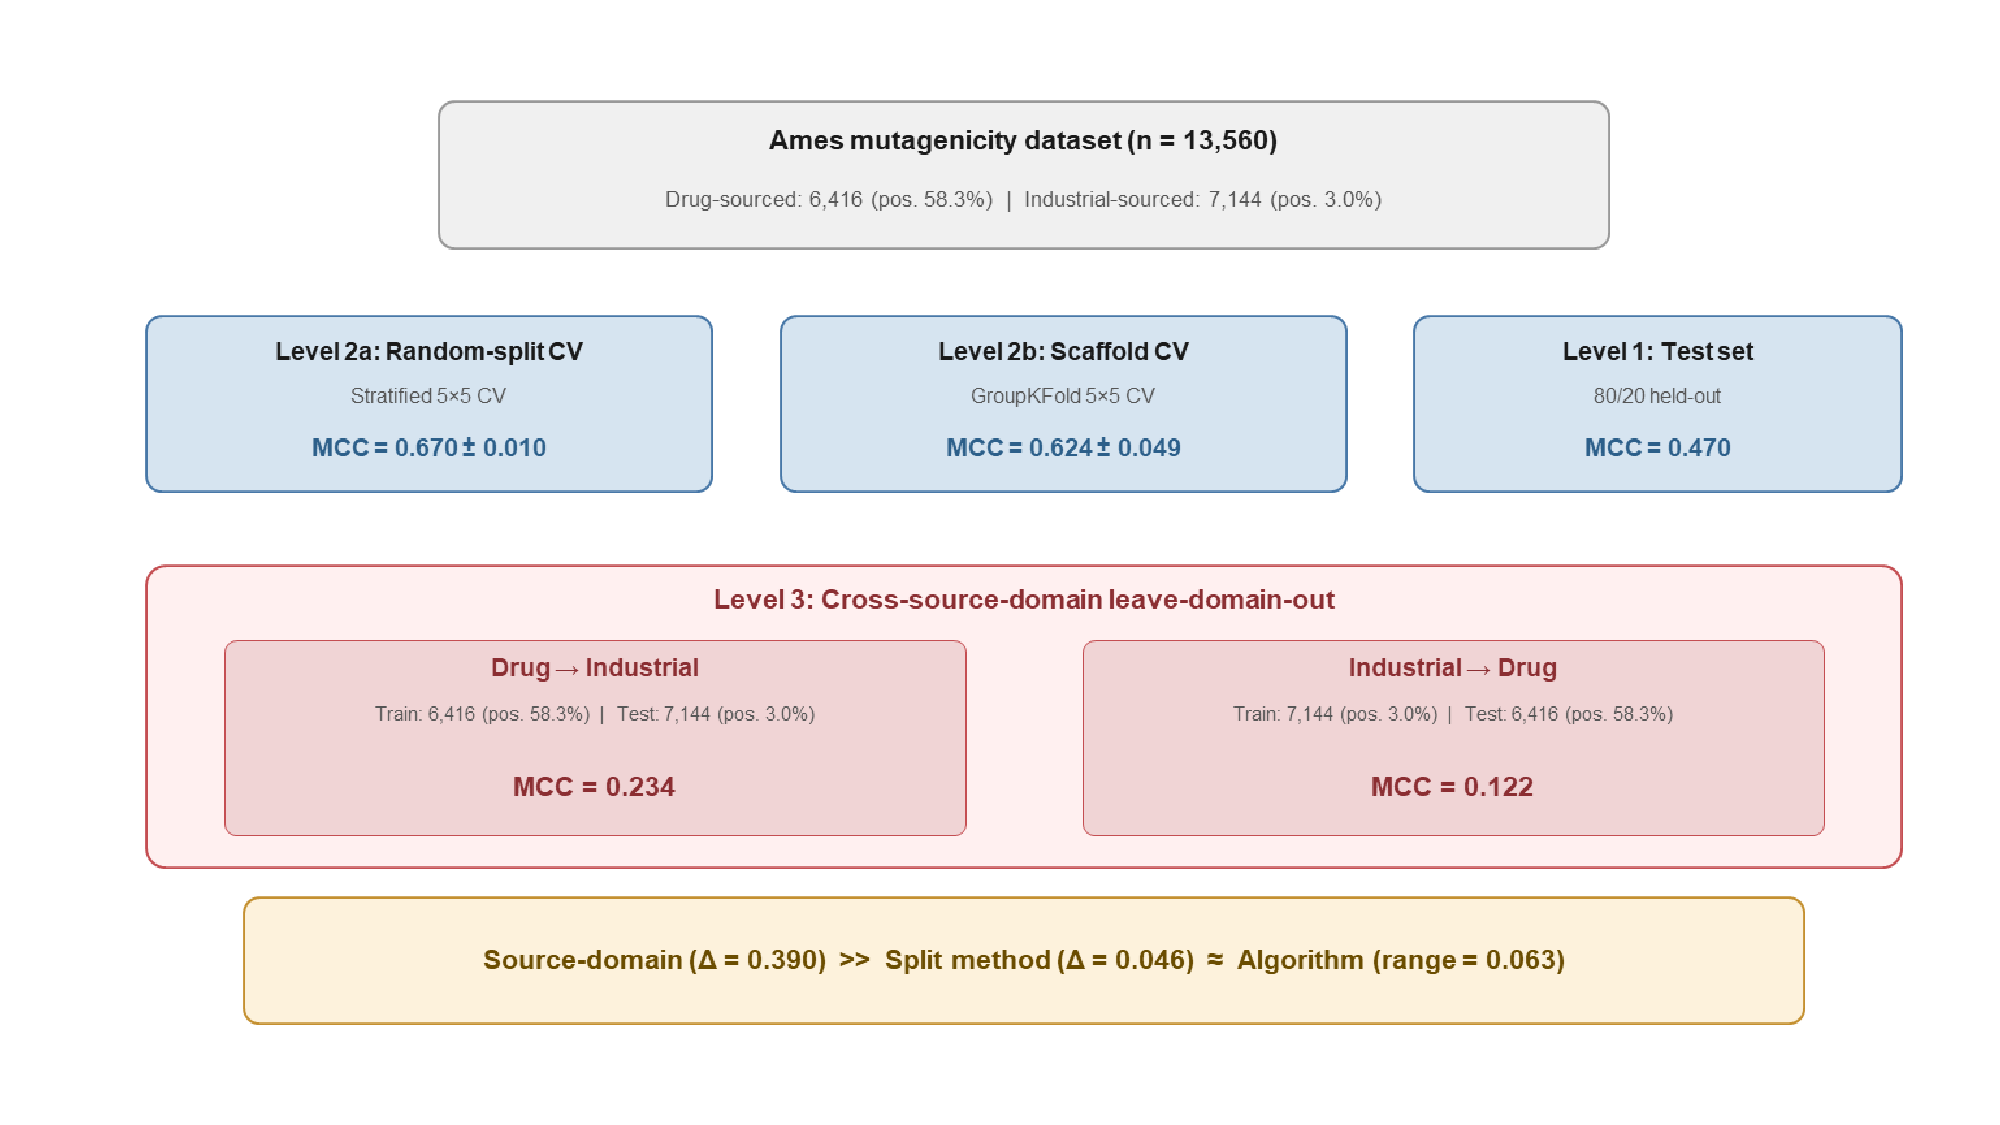
\includegraphics[width=\textwidth]{figures/figure1_framework.pdf}
\caption{Evaluation cascade framework. All levels use the same locked configuration (XGB, 
compact features, raw SMILES), enabling fair MCC comparison across evaluation methods.}
\label{fig:framework}
\end{figure}
